\documentclass[a4paper,10pt]{article}

%--------------------------PACKAGES--------------------------------------------

\RequirePackage{color,graphicx}
\usepackage[big]{layaureo} 				
\usepackage[usenames,dvipsnames]{xcolor}
\usepackage{amsfonts}
\usepackage{hyperref}
\usepackage{supertabular} 		
\usepackage{titlesec}				
\usepackage{xunicode,xltxtra,url,parskip} 	


%----------------------------SETTINGS-------------------------------------------
\defaultfontfeatures{Mapping=tex-text}
\definecolor{linkcolour}{rgb}{0,0.2,0.6}
\hypersetup{colorlinks,breaklinks,urlcolor=linkcolour, linkcolor=linkcolour}
\hyphenation{im-pre-se}
\newcommand{\icon}[1]{\includegraphics[height=0.5cm, width=0.5cm]{img/#1}}
\newcommand{\tvspace}{\footnotesize{}\\\multicolumn{2}{c}{}}

\setmainfont[
Path = font/,
SmallCapsFont = Fontin-SmallCaps.otf,
BoldFont = Fontin-Bold.otf,
ItalicFont = Fontin-Italic.otf
]
{Fontin.otf}


%--------------------BEGIN DOCUMENT--------------------------------------------
\begin{document}

\pagestyle{empty} % non-numbered pages

\font\fb=''[cmr10]'' %for use with \LaTeX command

%--------------------TITLE-----------------------------------------------------
\par{\centering
		{\Huge ANDY RUFASTO\\ \centering{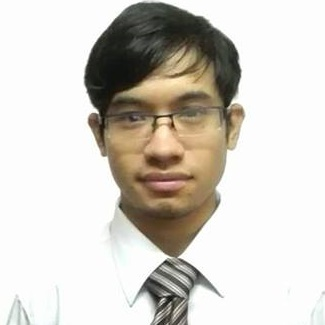
\includegraphics[width=3cm]{img/photo.jpg}
	}\bigskip\par} }


%--------------------SECTIONS--------------------------------------------------
\hfill\begin{minipage}{0.5\linewidth}
	(Última actualización Enero 2021)\\ 
	Descarga este documento:\\
 	\href{https://www.andyrufasto.cf/cv.pdf}{https://www.andyrufasto.cf/cv.pdf}
	\href{https://www.github.com/andyrufasto.cf/cv}{\LaTeX}
\end{minipage}

\section{Datos Personales}
	\hrule
	\begin{tabular}{rl}
    \textsc{DNI:}       & 70364804\\
    \textsc{Telefono:}  & 992 161 156\\
    \textsc{web:}       & \href{https://www.andyrufasto.cf}{https://www.andyrufasto.cf}\\
    \textsc{GitHub:}    & \href{https://www.github.com/andyrufasto}{@andyrufasto}\\
    \textsc{Linkedin:}  & \href{https://www.linkedin.com/in/andyrufasto/}{Andy Rufasto Chero}\\
    \textsc{email:}     & \href{mailto:andy@andyrufasto.cf}{andy@andyrufasto.cf}\\
				                & \href{mailto:andy.rufasto@unmsm.edu.pe}{andy.rufasto@unmsm.edu.pe}\\
	\end{tabular}

\section{Sobre Mí}
	\hrule

	Soy un joven estudiante de Economía, entusiasta del análisis y ciencia de datos, divulgador y contribuidor de software libre por lo que mis puntos fuertes son la capacidad de análisis y síntesis.

\section{Experiencia laboral}
	\hrule
	\begin{tabular}{r|p{11cm}}
		\textsc{2019}             & \textsc{DIGITADOR}\\
				                      & \textsc{Registro de Facturas, Cuadres}\\
				                      & \textbf{Consorcio Carolina S.A.C} \\
				                      & 261 - 2481 \\
				                      & Av. Bolivar 1831 - Pueblo Libre\\
															& \tvspace \\

		\textsc{2017}             & \textsc{ÁREA COMERCIAL}\\
				                      & \textsc{Compras, Cobranzas, proforma invoice, B2B}\\
				                      & \textbf{International Trading Company S.R.L.} \\
				                      & 261 - 2481 \\
				                      & Jr. Trujillo 546 utb primavera - Magdalena del Mar
	\end{tabular}

\newpage

\section{Cursos}
\hrule

	\begin{tabular}{r|p{11cm}}
 		\emph{Especialización}       & \textsc{Open Source Software Development, Linux and Git}\\
				                         & \textbf{The Linux Fundation}\\
		\textsc{2020}                & \href{https://www.coursera.org/verify/specialization/S9NNU5BM4SWU}{Certificado}\\
				                         & \tvspace \\

  	\emph{Curso}                 & \textsc{Introducción a Data Science: Programación Estadística con R}\\
				                         & \textbf{Universidad Nacional Autónoma de México}\\
		\textsc{2020}                & \href{https://www.coursera.org/verify/V6A9ZS2CMAP2}{Certificado}\\
	\end{tabular}


\section{Educación}
\hrule
	\begin{tabular}{r|p{11cm}}
					\emph{Cursando}      & \textsc{Economía}\\
														   & \textbf{Universidad Nacional Mayor de San Marcos, Lima} \\
					\textsc{2014}        & \emph{Pregrado}\\
 	                             & \tvspace \\

					\textsc{2010}        & \textsc{Secundaria} \\
														   & \emph{5139 \textbf{Las Colinas}, Callao} \\
                               & \tvspace \\

					\textsc{2009}        & Hardware de Computadoras\\
														   & \textsc{Centro de Tecnologías de la comunicación}\\
														   & \textbf{Universidad Nacional de Ingenieria, Lima}
	\end{tabular}


\section{Idiomas}
\hrule
	\begin{tabular}{rl}
 		\textsc{Español:} & Materno\\
 		\textsc{Inglés:}  & Intermedio\\
	\end{tabular}

\section{Conocimientos informáticos}
\hrule

\begin{minipage}[b]{\textwidth}
\begin{minipage}[b]{0.5 \textwidth}
	Lenguajes de Programación:
	\begin{itemize}
				\item[--] \icon{gnubash.png}\textsc{Bash/Shell}
				\item[--] \icon{python.png}\textsc{Python}
				\item[--] \icon{r.png}\textsc{R}
				\item[--] \icon{julia.png}\textsc{Julia}
				\item[--] \icon{octave.png}\textsc{GNU Octave/Matlab}
\end{itemize} \end{minipage} \hfill
\begin{minipage}[b]{0.5 \textwidth}
	Programas Estadísticos:
	\begin{itemize}
				\item[--] \textsc{SPSS}
				\item[--] \textsc{Eviews}
				\item[--] \textsc{Stata}
	\end{itemize}
	Sistemas Operativos:
	\begin{itemize}
					\item[--] \icon{linux.png} \textsc{Linux} 
					\item[--] \icon{windows.png} \textsc{Windows}
	\end{itemize}
\end{minipage}\end{minipage}


\begin{minipage}[b]{\textwidth}
\begin{minipage}[b]{0.5 \textwidth}
	Lenguajes de marcado:
	\begin{itemize}
					\item[--]  \icon{latex.png}\textsc{Latex}
					\item[--]  \icon{html5.png}\textsc{HTML}
					\item[--]  \icon{markdown.png}\textsc{Markdown}
	\end{itemize}
	Control de versiones:
	\begin{itemize}
					\item[--] \icon{git.png}\textsc{git}
\end{itemize} \end{minipage} \hfill
 \begin{minipage}[b]{0.5 \textwidth}
	Office:
 \begin{itemize}
				 \item[--] \icon{microsoftexcel.png}\textsc{excel}          
				 \item[--] \icon{microsoftword.png} \textsc{Word}  
				 \item[--] \icon{microsoftpowerpoint.png}\textsc{PowerPoint}
				 \item[--] \icon{mysql.png}\textsc{SQL} 
 \end{itemize}
\end{minipage}\end{minipage} 

\newpage

\section{Projectos Publicados}
\hrule
\begin{tabular}{r|p{11cm}}
  \emph{web}                   & \textsc{web\_andyrufasto}\\
	                             & \textbf{Página web personal sobre ecnomía y Linux} \\
	\textsc{GPL-3.0}             & \href{https://www.andyrufasto.cf}{www.andyrufasto.cf}\\
				                       & \tvspace \\

  \emph{Configuraciones}       & \textsc{Lain-Dotfiles}\\
	                             & \textbf{Configuraciones de Unix Software} \\
	\textsc{GPL-3.0}             & \href{https://www.andyrufasto.cf}{www.andyrufasto.cf}
															
\end{tabular}

\end{document}
